% !TEX root =  ../../thesis.tex

\chapter{Analysis of blood donor data set}
\label{ch : blood_donor}
 
 In this chapter we will present the analysis of the blood donor data set \citep{nasserinejad_prevalence_2015} using the Bayesian heterogeneity model. The data set consists of 1595 male blood donors who donated blood multiple times over a period of many years. Each time they visited the donation center, the following information was noted: Season in which blood was donated (Cold/Hot), Volume of blood donated (ml), age at the time of donation (years), a binary indicator Donate (yes/no) specifying if the donor was allowed to donate the blood, Hemoglobin (Hb) of the patient at the time of donation, and the date of visit. \citet{nasserinejad_predicting_2013,nasserinejad_prevalence_2015,nasserinejad_prediction_2016} have analyzed this data set extensively using transition models, mixed models, growth mixture models and latent class mixed effects transition models. The analysis was used to predict the Hb level of donors so that they are invited for donation at an optimal time, i.e. when their Hb levels are not too low because of the previous donations and other factors.\\

 For the purpose of this thesis we did not use the entire data set of 1595 patients as Bayesian computation for heterogeneity model using the entire data set required large amount of computational resources. Instead we used a simple random sample of the data consisting of 250 subjects.

\section{Motivation for analysis with Bayesian heterogeneity model}
 In the analysis using growth mixture models \citet{nasserinejad_prevalence_2015} found 4 different underlying subpopulations in the data set. Firstly, those which had a relatively stable Hb level over donations. Secondly, those which had a higher Hb level than those in category 1 and showed a slow decline of Hb level over donations. Thirdly, those which showed a moderately sharp decline in Hb level over donations, and lastly those which showed a steep decline in Hb levels despite beginning at high initial Hb levels. Because of the presence of different subpopulations, a single methodology to decide the time of next blood donation for subjects from all subpopulations may not be effective. The aim of applying the Bayesian heterogeneity model to this dataset is to provide an alternative modeling framework for such data sets.

\section{Frequentist analysis}
\label{sec : frequentist_blood_donor}
We began with a frequentist analysis of the blood donor data set to select the right mean structure for our models ahead. This was necessary because omitting a required covariate in the mean structure can lead to incorrect estimates of the covariance matrix. Secondly, a frequentist analysis provided us good starting values for the various parameters in our model. Thirdly we could check if the Bayesian analysis results are consistent with the frequentist analysis results. For the random effects structure we considered a model with both random intercept and random slope. For the choice of random slope we selected the number of donations in last 2 years as that was deemed as a suitable variable for random slope by \citet{nasserinejad_prevalence_2015}. For selecting the mean structure we did F-tests and likelihood ratio tests based on ML. We found the following mean structure to be suitable.

\begin{equation}
\label{eq : blood_donor_model}
\begin{split}
\boldsymbol{y}_{ij} = \beta_0 + \beta_1*\text{Age}_{ij} + \beta_2*\text{Season}_{ij} + \beta_3*\text{Donate}_{ij} + \beta_4*\text{TSPD}_{ij}\\
+ \beta_4*\text{\#donationLast2Years}_{ij} + \beta_5*\text{\#donationLast2Years}_{ij}*\text{TSPD}_{ij}\\
+ \beta_6*\text{\#donationLast2Years}_{ij}*\text{Donate}_{ij} + \beta_7*\text{\#donationLast2Years}_{ij}^2\\
+ b_0 + b_1 * \text{\#donationLast2Years}_{ij} + \varepsilon_{ij}
\end{split}
\end{equation}

where, Age and TSPD have been standardized to have mean 0 and variance 1, $\text{\#donationLast2Years}_{ij}$ have been downscaled by a factor of 100 so that the random slope variance scale is upscaled. Similarly the intercept we used was 0.1, thus upscaling the random intercept variance. We will now present the fixed effect and random effect variance estimates of equation above. It is important to note that this model assumes a single multivariate normal distribution for the distribution of random effects.

\begin{table}[!htb]
\centering
\caption{Table of frequentist fixed effects estimates for model \ref{eq : blood_donor_model}}
\label{table : frequentist_fixed effects}
\begin{tabular}{@{}lrr@{}}
\toprule
Effect ($\beta$) & Estimate & Standard Error \\ \midrule
intercept & 94.121 & 0.429 \\
Age & -0.086 & 0.026 \\
\#donationLast2Years & -7.265 & 1.555 \\
TSPD & -0.036 & 0.015 \\
Season (Hot) & -0.080 & 0.016 \\
Donate (TRUE) & 0.155 & 0.037 \\
\#donationLast2Years * TSPD & 0.020 & 0.006 \\
\#donationLast2Years * Donate & 4.689 & 0.995 \\
$\text{\#donationLast2Years}^2$ & -52.796 & 15.237 \\ \bottomrule
\end{tabular}

\begin{tabular}{@{}lr@{}}
\toprule
Cov Parm & Estimate \\ \midrule
$G[1,1]$ & 19.971 \\
$G[1,2]$ & -14.266 \\
$G[2,2]$ & 40.183 \\
$\sigma^2$ & 0.201 \\ \bottomrule
\end{tabular}
\end{table}

\section{Bayesian analysis}
We next fitted the same model with Bayesian approach, although we also fitted mixtures with more number of components in the random effects. We first began with the approach in \ref{subsec : ds_description} to get a rough idea of the number of components. Figure \ref{fig : rough_idea_blood_donor} shows that there could be perhaps 1 component, or if there are more they have small number of subjects. Besides as we know these values overestimate the exact random effects thus if there are more than 1 component, we will have to use a slightly higher value for the hyperparameter of the Dirichlet prior in such case. We used $\text{Dir}(2, 2,...2)$. Firstly in a mixture of only 1 component, i.e. no mixture case had the same mean value for fixed effect and random effect posterior distributions.\\

\begin{figure}
	\centering
	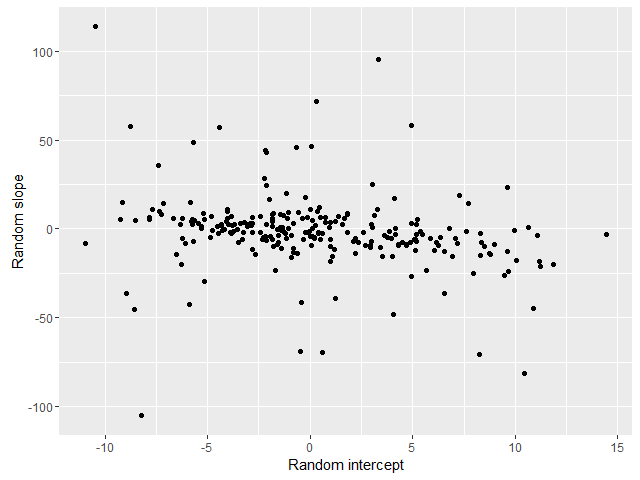
\includegraphics[scale=0.5]{mainmatter/chapter_6_blood_donor/rough_estimate_random_effects.png}
	\caption{Rough estimate $\tilde{\boldsymbol{b}_i}$ for random effects}
	\label{fig : rough_idea_blood_donor}
\end{figure}

To do the Bayesian analysis we ran 150000 iterations with a thinning of 100 and burn-in of 25000 iterations. For chains with higher number of components we used 200000 iterations with a thinning of 150. For each of the resulting MCMC chains we calculated the various definitions of definitions given in section \ref{sec : dic}, the results of which are presented in Table \ref{table : dic_blood_donor}. In the simulation study we observed that $\text{DIC}_4$ was the most reliable of the DIC's and so we will discuss it first. It seems that there are not more than 2-3 components. The difference between DIC of mixture of 1 component and of 2 components is much larger than that between 2 and 3 components. To further verify this we used posterior predictive checks. However instead of randomly generating number of donations in last 2 years we sampled them from the subjects which were not considered for analysis due to computational restrictions. As shown in Figure \ref{fig : ppc_blood_donor_3comp} to \ref{fig : ppc_blood_donor_5comp}, it is clear that 3 or more components are an overfit. Secondly we can see that the posterior predictive distribution of the test statistic overlaps the distribution of test statistic with the sample data. Thus we will stick to the choice of 2 components.\\

\begin{table}[!htb]
\centering
\caption{DIC for blood donor data set}
\label{table : dic_blood_donor}
\begin{tabular}{@{}rrrrrrr@{}}
\toprule
\# Comp Fitted & $\text{DIC}_1$ & $\text{DIC}_2$  & $\text{DIC}_3$  & $\text{DIC}_4$  & $\text{DIC}_5$  & $\text{DIC}_6$  \\ \midrule
1 comp & 4817 & 4816 & 4818 & 7077 & 7532 & 4353 \\
2 comp & 4810 & 4804 & 4814 & 7040 & 7492 & 4339 \\
3 comp & 4744 & 4777 & 4814 & 7032 & 7458 & 4344 \\
4 comp & 4608 & 4723 & 4814 & 7031 & 7360 & 4332 \\
5 comp & 4461 & 4459 & 4818 & 7031 & 7108 & 4327 \\ \bottomrule
\end{tabular}
\begin{tabular}{@{}rrrrrrr@{}}
\toprule
\# Comp Fitted & ${\text{p}_\text{D}}_1$ & ${\text{p}_\text{D}}_2$ & ${\text{p}_\text{D}}_3$ & ${\text{p}_\text{D}}_4$ & ${\text{p}_\text{D}}_5$ & ${\text{p}_\text{D}}_6$ \\ \midrule
1 comp & 13 & 12 & 15 & 13 & 468 & 302 \\
2 comp & 17 & 11 & 21 & 19 & 471 & 281 \\
3 comp & -48 & -15 & 22 & 25 & 451 & 284 \\
4 comp & -183 & -67 & 23 & 30 & 360 & 272 \\
5 comp & -334 & -336 & 23 & 28 & 104 & 269 \\ \bottomrule
\end{tabular}
\end{table}

\begin{figure}[!htb]
\centering
\begin{subfigure}[b]{0.4\textwidth}
		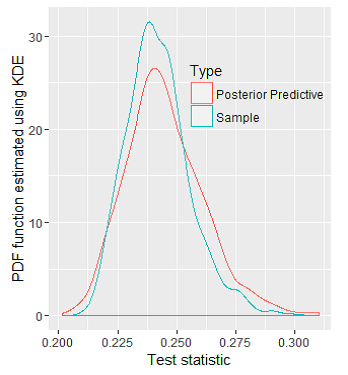
\includegraphics[width=\textwidth]{mainmatter/chapter_6_blood_donor/ppc_1comp.png}
        \caption{\label{fig : ppc_blood_donor_1comp}1 components fitted for blood donor data set}
	\end{subfigure}
	\begin{subfigure}[b]{0.4\textwidth}
		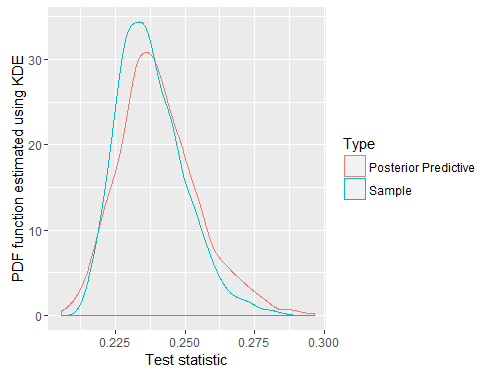
\includegraphics[width=\textwidth]{mainmatter/chapter_6_blood_donor/ppc_2comp.png}	
          \caption{\label{fig : ppc_blood_donor_2comp}2 components fitted for blood donor data set}
	\end{subfigure}
	\begin{subfigure}[b]{0.4\textwidth}
		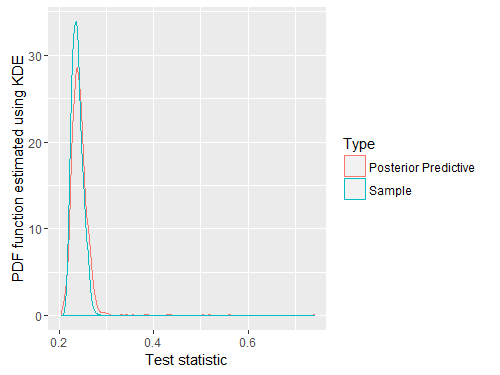
\includegraphics[width=\textwidth]{mainmatter/chapter_6_blood_donor/ppc_3comp.png}	
          \caption{\label{fig : ppc_blood_donor_3comp}3 components fitted for blood donor data set}
	\end{subfigure}
	\begin{subfigure}[b]{0.4\textwidth}
		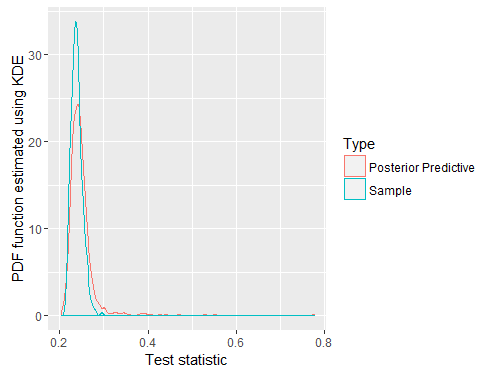
\includegraphics[width=\textwidth]{mainmatter/chapter_6_blood_donor/ppc_4comp.png}	
          \caption{\label{fig : ppc_blood_donor_4comp}4 components fitted for blood donor data set}
	\end{subfigure}
	\begin{subfigure}[b]{0.4\textwidth}
		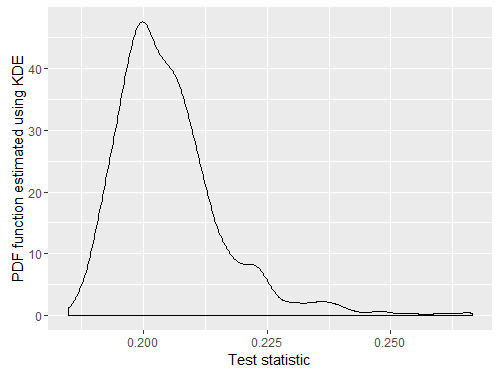
\includegraphics[width=\textwidth]{mainmatter/chapter_6_blood_donor/ppc_5comp.png}	
          \caption{\label{fig : ppc_blood_donor_5comp}5 components fitted}
	\end{subfigure}
	
	\caption{PDF function of $T(\boldsymbol{\tilde{r}})$ estimated using KDE for blood donor data set. The red line shows the value of the test statistic $T(\boldsymbol{r})$ based on the observed data.}
	\label{fig : ppc_blood_donor}    
\end{figure} 

\subsection{Parameter estimates}
For the 2 components we will now present the summary of the parameter estimates. Firstly in Figure \ref{fig : eta_blood_donor} we can see that the two components are equal in weight distribution. However the posterior of the weights is bimodal for both of them. Although this is usually a sign of label switching....hmm but my means don't seem to be having label switching. need to check this.

\begin{figure}[!htb]
\centering
\begin{subfigure}[b]{0.4\textwidth}
		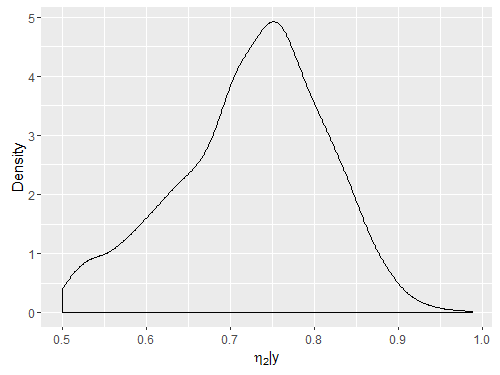
\includegraphics[width=\textwidth]{mainmatter/chapter_6_blood_donor/eta1.png}
        \caption{\label{fig : eta_blood_donor_1} Weight for the first component $\eta_1$}
	\end{subfigure}
	\begin{subfigure}[b]{0.4\textwidth}
		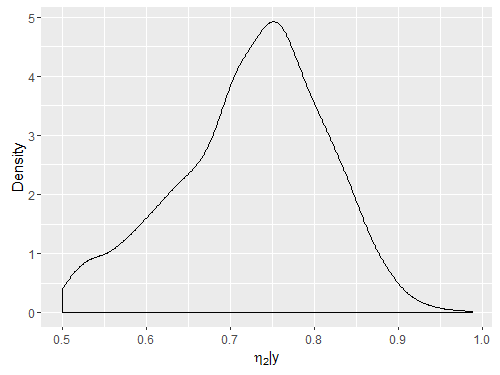
\includegraphics[width=\textwidth]{mainmatter/chapter_6_blood_donor/eta2.png}	
          \caption{\label{fig : eta_blood_donor_2}Weight for the second component $\eta_2$}
	\end{subfigure}	
	\caption{Weight distribution for the components of the mixture of random effects.}
	\label{fig : eta_blood_donor}    
\end{figure} 

\begin{figure}[!htb]
\centering
\begin{subfigure}[b]{0.4\textwidth}
		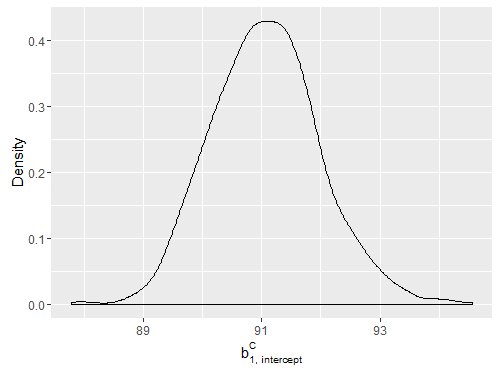
\includegraphics[width=\textwidth]{mainmatter/chapter_6_blood_donor/b11.png}
        \caption{\label{fig : mu_blood_donor_11} Intercept location for the first component $b_{1, \text{intecept}}$}
	\end{subfigure}
	\begin{subfigure}[b]{0.4\textwidth}
		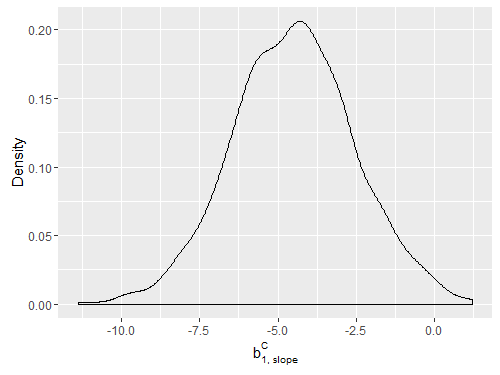
\includegraphics[width=\textwidth]{mainmatter/chapter_6_blood_donor/b12.png}	
          \caption{\label{fig : mu_blood_donor_12}Slope location for the first component $b_{1, \text{slope}}$}
	\end{subfigure}
	\begin{subfigure}[b]{0.4\textwidth}
		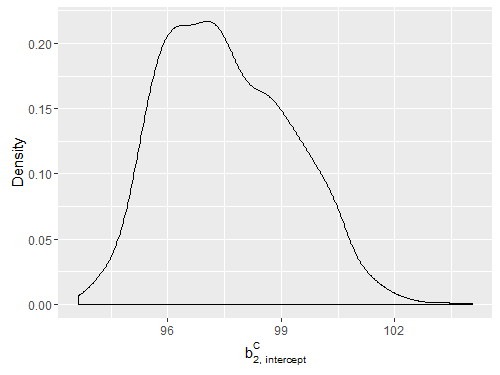
\includegraphics[width=\textwidth]{mainmatter/chapter_6_blood_donor/b21.png}	
          \caption{\label{fig : mu_blood_donor_21}Intercept location for the second component $b_{2, \text{intecept}}$}
	\end{subfigure}	
	\begin{subfigure}[b]{0.4\textwidth}
		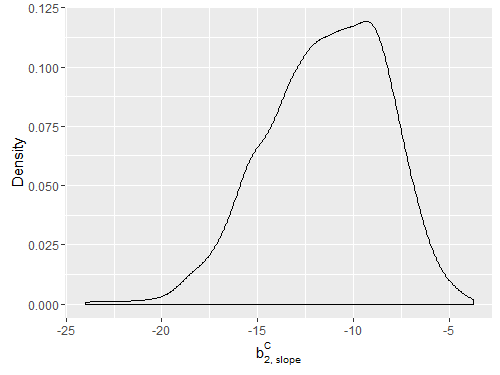
\includegraphics[width=\textwidth]{mainmatter/chapter_6_blood_donor/b22.png}	
          \caption{\label{fig : mu_blood_donor_22}Slope location for the second component $b_{2, \text{slope}}$}
	\end{subfigure}	
	\caption{The location parameters for the components of the mixture of random effects.}
	\label{fig : mu_blood_donor}    
\end{figure} 

\begin{figure}[!htb]
\centering
\begin{subfigure}[b]{0.4\textwidth}
		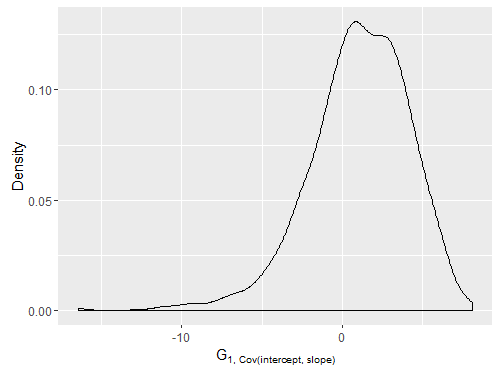
\includegraphics[width=\textwidth]{mainmatter/chapter_6_blood_donor/G11_1.png}
        \caption{\label{fig : cov_blood_donor_11_1} Intercept variance for the first component}
	\end{subfigure}
	\begin{subfigure}[b]{0.4\textwidth}
		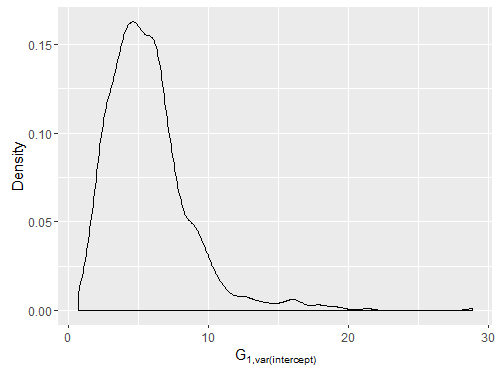
\includegraphics[width=\textwidth]{mainmatter/chapter_6_blood_donor/G12_1.png}	
          \caption{\label{fig : cov_blood_donor_12_1} Covariance between intercept and slope for the first component}
	\end{subfigure}
	\begin{subfigure}[b]{0.4\textwidth}
		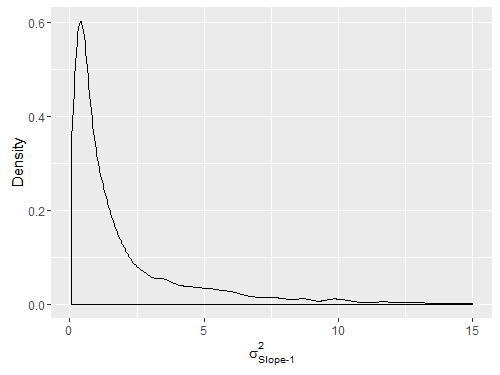
\includegraphics[width=\textwidth]{mainmatter/chapter_6_blood_donor/G22_1.png}	
          \caption{\label{fig : cov_blood_donor_22_1}Slope variance for the first component}
	\end{subfigure}	
	\begin{subfigure}[b]{0.4\textwidth}
		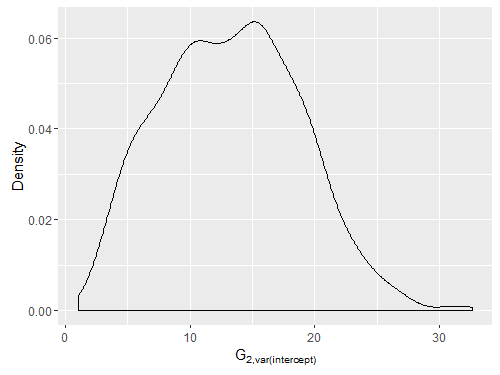
\includegraphics[width=\textwidth]{mainmatter/chapter_6_blood_donor/G11_2.png}
        \caption{\label{fig : cov_blood_donor_11_2} Intercept variance for the second component}
	\end{subfigure}
	\begin{subfigure}[b]{0.4\textwidth}
		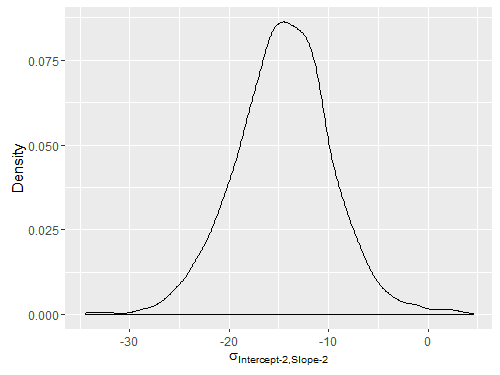
\includegraphics[width=\textwidth]{mainmatter/chapter_6_blood_donor/G12_2.png}	
          \caption{\label{fig : cov_blood_donor_12_2} Covariance between intercept and slope for the second component}
	\end{subfigure}
	\begin{subfigure}[b]{0.4\textwidth}
		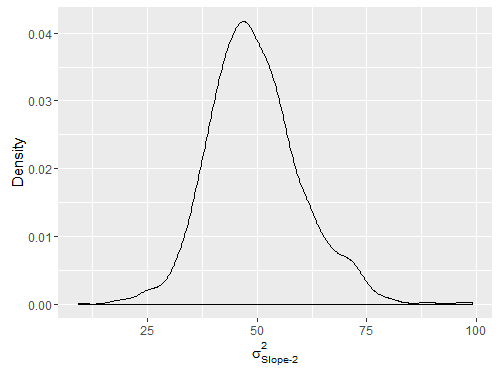
\includegraphics[width=\textwidth]{mainmatter/chapter_6_blood_donor/G22_2.png}	
          \caption{\label{fig : cov_blood_donor_22_2}Slope variance for the second component}
	\end{subfigure}	


	\caption{The variance covariance parameters for the components of the mixture of random effects.}
	\label{fig : cov_blood_donor}    
\end{figure} 